\section{Introduction}\label{chap4-sec:intro}
 Federated analytics enable a data analyst to gather useful information from data distributed across multiple users \textit{without} centrally pooling the data. An important class of tasks in federated analytics  is computing statistics over graph data, which has wide-spread applications ranging from market value prediction~\cite{matsunaga2019exploring}, fake news detection~\cite{benamira2019semi} to drug development~\cite{gaudelet2021utilizing}.  Usually, the graph encodes sensitive user information, such as social network data, which raises privacy concerns.  For instance, a mobile phone company might be interested in calculating statistics over the graph of call history which reveals an user's social interactions. To this end, local differential privacy (\ldp) is currently the most popular model for achieving data privacy for federated analytics. %\ldp~has been deployed by major commercial organizations, such as Google~\cite{Rappor1,Rappor2}, Apple~\cite{Apple} and Microsoft~\cite{Microsoft}.\textcolor{white}{t\symfootnote{The first two authors have made equal contributions.}}

%Unfortunately, \ldp~brings forth a host of challenges. 

The distributed nature of \ldp, however, leaves the door open for poisoning attacks. For example, an adversary can inject fake users into the system or compromise the accounts of real users to run untrusted applications on user devices. Consequently, there is no guarantee that these users will comply with the \ldp~protocols. The adversary can send carefully crafted malformed data from these non-compliant users and skew statistical estimates, including those involving only honest users. 
%Additionally, such poisoning attacks can tamper with statistics that pertain to only the honest users. 
\begin{figure}
    \centering
    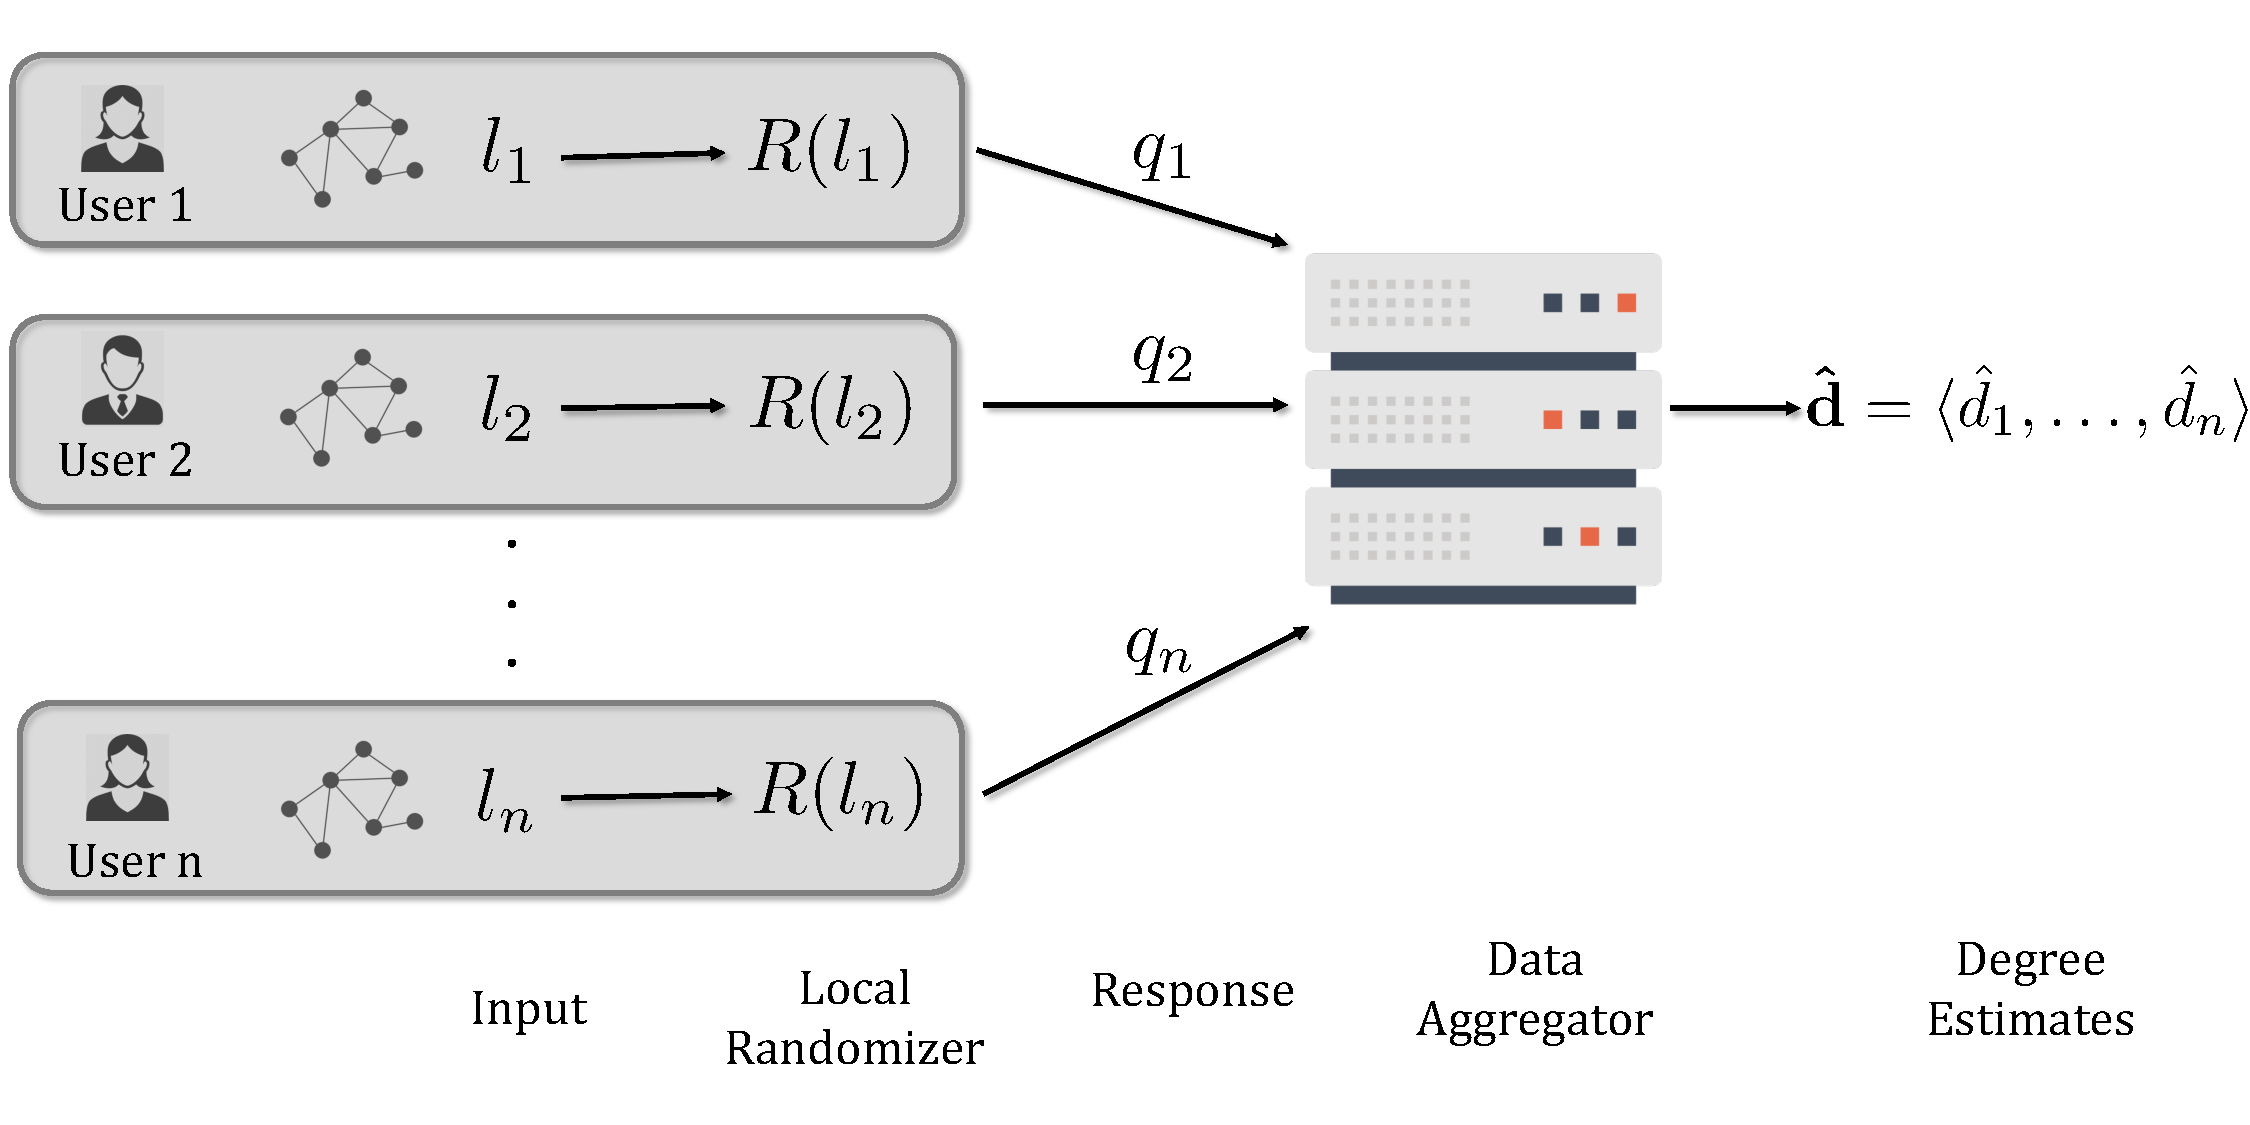
\includegraphics[width=0.78\columnwidth]{graph_pic_1_new.pdf}
     \vspace{-0.3cm}
  \caption{Graph analysis in the \ldp~setting}
    \label{chap4-fig:setting}   
    \vspace{-1cm}
\end{figure}

Prior work, which focuses on tabular data~\cite{Cheu21,Cao_USENIX21,Li22}, finds that  poisoning attacks can be carried out against naive \ldp{} protocols. However, the impact of poisoning under \ldp{} for graph analysis is largely unexplored. In this paper, we initiate a formal study on the impact of such poisoning attacks on \ldp{} protocols for graph statistics. We focus on the task of degree estimation, one of the most fundamental tasks in graph analysis. 

A real-world use-case for a poisoning attack is as follows. Suppose a data analyst is interested in hiring the most influential nodes (users) of a graph for marketing and uses a node's degree as its measure of influence.  Here, an adversary might want to promote a specific malicious node (user) to be selected as an influencer or prevent an honest node from being selected as an influencer. Concretely, suppose a single malicious user wants to (falsely) get themselves selected as the most influential node. If the \ldp~protocol used is the Laplace mechanism, where each user directly submits their (noisy) degree to the analyst (Fig. \ref{chap4-fig:setting}), then the malicious user can lie flagrantly and report their degree to be $n-1$. This can skew the response by as much as the number of users!

%A near-optimal solution to degree-estimation with \ldp~is the Laplace mechanism where every user directly submits their (noisy) degree to the analyst (Figure \ref{chap4-fig:setting}). If this is the pthe malicious user can hack into the mobile application collecting the data and manipulate the response arbitrarily. Consequently, they can flagrantly lie and respond with $n-1$,  



 %Consider a data analyst interested in hiring the most influential user in a graph for marketing. To do so, the analyst asks each node to release their list of friends (edges) privately. Unfortunately, any estimates based on this protocol are susceptible to data poisoning; for example, an adversary might create fake accounts with whom they are friends or lie about being friends with real users. The second attack is particularly devastating --- the adversary could report that he is friends with everyone in the graph! Finally, an adversary may try to reduce an honest user's influence by compromising their friends and reporting no friendship. These attacks are unique to the graph setting, there is no analogue in the \ldp{} literature on tabular data.

We  address this challenge and design degree estimation protocols that are robust to poisoning attacks. Our algorithms are based on the key observation that graph data is naturally redundant -- the information about an edge $e_{ij}$ is shared by both users $\DO_i$ and $\DO_j$. Leveraging this observation, we propose robust protocols based on two new ideas. First, we use \textit{distributed information} -- we collect the information about each edge from \textit{both} users. The second idea is to \textit{verify} -- the data analyst can verify the consistency of the collected information by leveraging its redundancy. Specifically, as long as at least one of $\DO_i$ or $\DO_j$ is honest, the analyst can check for consistency\footnote{For the ease of exposition, we disregard errors due to machine failures.} between the two bits obtained from $\DO_i$ and $\DO_j$ and detect malicious behavior. 

If there are at most $m$ malicious users, then with no privacy, the data analyst could flag malicious users as those with more than $m$ edge inconsistencies in their reported edges since this is beyond a tolerable number of inconsistencies for an honest user. However, \ldp~requires randomization which makes the user's reports probabilistic. Consequently, the aforementioned simple consistency check cannot be applied directly to \ldp~protocols. We mitigate this challenge by proposing edge inconsistency confidence bounds under \ldp~which guarantees detection of malicious users without misclassifying the honest ones. Using our edge consistency checks we design novel degree estimation protocols under \ldp~which are robust to poisoning attacks.

%To this end, we design novel degree estimation protocols that enable a data analyst to employ consistency checks and detect malicious users even under \ldp. 
 

%We observe that \ldp~makes a degree estimation protocol more vulnerable to poisoning -- the impact of poisoning is worse when the adversary can directly poison their (noisy) responses (Fig. \ref{chap4-fig:response}), rather than their input data (Fig. \ref{chap4-fig:input}).  The former utilizes the characteristics of \ldp~while the latter is independent of \ldp.





In summary, we are the \textit{first} to study the impact of poisoning  on \ldp~degree estimation for graphs. Our main contributions are: 
\squishlist
    \item We propose a formal framework for analyzing the robustness of a protocol. %The framework quantifies the impact of poisoning attacks on both honest and malicious   users. 
Specifically, we measure the robustness along two dimensions, \textit{correctness} (for honest users) and \textit{soundness} (for malicious users). Intuitively, good correctness means that the protocol is accurate for honest users, and good soundness means that it can detect/restrict malicious users. %Hence, a protocol which has both properties is robust to poisoning attacks.
\item Based on the proposed framework, we study the impact of poisoning attacks on private degree estimation in the \ldp~setting. The attacks can be classified into two types: $(1)$ input poisoning attacks  where the adversary does not have access to implementation of the \ldp~protocol and can only falsify their input data (Fig. \ref{chap4-fig:input}), and $(2)$ response poisoning attacks where the adversary can tamper with the \ldp~implementation and directly manipulate the (noisy) responses of the \ldp~protocol (Fig. \ref{chap4-fig:response}). The former is independent of \ldp~while the latter utilizes the characteristics of \ldp. We observe that \ldp~makes a degree estimation protocol more vulnerable to poisoning -- the impact of a response poisoning attack can be worse than that of any input poisoning attack. 
\item Leveraging the natural redundancy in graph data, we design robust degree estimation protocols under \ldp~that significantly reduce the impact of adversarial poisoning and compute degree estimates with high accuracy (Table \ref{chap4-tab:results}).
\item We evaluate our proposed robust degree estimation protocols under poisoning attacks on real-world datasets to demonstrate their efficacy in practice. We observe that even a relatively
small number of malicious parties $(m = 1\% )$ can stage significantly damaging poisoning attacks. This demonstrates the
practical threat of such attacks. Nevertheless, our empirical results show that our proposed protocols are
able to thwart poisoning attacks
even with a large number of malicious users $(m = 37.5\%)$.
\squishend



%We focus on the task of degree estimation and propose protocols provide formal robustness guarantees against data poisoning attacks that significantly reduce the impact of poisoning and compute degree estimates with high accuracy. The key observation Leveraging the redundancy in graph data, we design robust degree estimation protocols under \ldp~that significantly reduce the impact of adversarial poisoning and compute degree estimates with high accuracy. Our empirical 
  


%In this paper, we initiate a formal study of the impact of data poisoning on \ldp{} protocols for graph statistics. We focus on the task of degree estimation, one of the most fundamental tasks in graph analysis which can be used to estimate  node influence. We formalize what it means for an \ldp{} graph protocol to be accurate and robust to data poisoning attacks. Specifically, we permit a protocol to flag a malicious user, and robustness means that a malicious user is either flagged or receives an accurate estimate. Consistent with the attacks described above, under our definitions, the naive randomized response protocol is accurate but not robust. 


%\par We observe that data poisoning can significantly skew the results of standard \ldp~protocols. For instance, consider the Laplace mechanism where every user directly submits their (noisy) degree to the analyst (Fig. \ref{chap4-fig:setting}). However, a malicious user can flagrantly lie and respond with $n-1$,  skewing their response by as much as the number of users. We  address this challenge and design robust degree estimation protocols. Our protocols are based on the key observation --   graph data is naturally redundant. Specifically, the presence (or absence) of edge $e_{ij}$ is shared by both users $\DO_i$ and $\DO_j$. This introduces data redundancy which we leverage to provide robustness -- as long as at least one of $\DO_i$ or $\DO_j$ is honest, the analyst can check for consistency between the two bits obtained from $\DO_i$ and $\DO_j$. We illustrate this using the following degree-estimation protocol. For the ease of exposition, we assume no privacy. Consider a protocol where the users send in their (true) adjacency lists. Here for every edge $e_{ij}$, the analyst receives two copies of the same bit from users $\DO_i$ and $\DO_j$ -- in case there is inconsistency\footnote{For the ease of exposition, we disregard errors due to machine failures.} in the two reported bits, the analyst can safely conclude that one party is malicious and act accordingly. Thus, we see that the natural data redundancy in graphs can be leveraged to perform robust data analysis. However, \ldp~requires randomization which makes the user's reports probabilistic. Consequently, the aforementioned simple consistency check cannot be applied to \ldp~protocols.  To this end, we design novel degree estimation protocols that enable a data analyst to employ consistency checks and detect malicious users even under \ldp. Our proposed protocols provide formal robustness guarantees against data poisoning attacks that significantly reduce the impact of poisoning and compute degree estimates with high accuracy. 

\begin{comment}In summary, we make the following contributions:
\squishlist
  \item 
  \item We propose a formal framework for analyzing the robustness of a protocol. The framework quantifies the impact of poisoning attacks on both honest and malicious   users. 
 \item Based on the proposed framework, we study the impact of poisoning attacks on private degree estimation in the \ldp~setting. We observe that \ldp~makes a degree estimation protocol more vulnerable to poisoning -- the impact of poisoning is worse when the adversary can directly poison their (noisy) responses (Figure \ref{chap4-fig:response}), rather than their input data (Figure \ref{chap4-fig:input}).  The former utilizes the characteristics of \ldp~while the latter is independent of \ldp.

 
  
  \item Leveraging the redundancy in graph data, we design robust degree estimation protocols under \ldp~that significantly reduce the impact of adversarial poisoning and compute degree estimates with high accuracy. 
  
    \item We evaluate our proposed robust degree estimation protocols under poisoning attacks on real-world datasets to demonstrate their efficacy in practice. We observe that even with a with a smasll () cab have significantly 
\squishend
\end{comment}
%In our paper, we first propose a formal framework for analyzing the robustnessof an algorithm under an attack. We study the robustness of a naive algorithm for estimating degrees under two common attacks against \ldp{} protocols. 

%Second, utilizing redundancy in graph data, we design protocols protocols utilizing the redundancy in graphs which also satisfy \ldp{}. Our results demonstrate the following:  (1) that adversarial manipulation becomes worse when the adversary is able to manipulate their (noisy) response, rather than their input data, and (2) that it is possible to leverage the redundancy in graph data to significantly reduce adversarial manipulation.In graphs, redundancy may be used to reduce the influence a malicious party has over \ldp{} protocols. If allowed to return $\bottom$ when auser is believed to be adversarial, a protocol is able to limit theadvantage of an adversary to much below what is achieved by naive approaches.

%\ji{ TODO: Table of results}
\begin{table*}
\centering
\begin{tabular}{|c|ccc|ccc|c|}
\hline 
\multirow{2}{*}{Protocol} & \multicolumn{3}{|c|}{Response Poisoning} & \multicolumn{3}{|c|}{Input Poisoning} & \multirow{2}{*}{Privacy Guarantee} \\
& Correctness & Soundness & & Correctness & Soundness & & \\ \hline
\RLap & $(\tO(\frac{1}{\epsilon}), \delta)$ & $(n-1)$-tight& Thm.~\ref{chap4-thm:response:laplace}& $(\tO(\frac{1}{\epsilon}), \delta)$ & $(n-1, \frac{1}{2})$ & Thm.~\ref{chap4-thm:input:laplace} & $\epsilon$-Edge \ldp\\ \hline 
\DegRRNaive & $(\tO(m + \frac{m}{\epsilon} + \frac{\sqrt{n}}{\epsilon}), \delta)$ & $(n-1)$-tight  & Thm.~\ref{chap4-thm:response:naive} & $(\tO(m + \frac{\sqrt{n}}{\epsilon}), \delta)$ & $(n-1, \frac 1 2)$  & Thm.~\ref{chap4-thm:input:naive} & $\epsilon$-Edge \ldp\\ \hline
\DegRRCheck & $(\tO(m + \frac{m}{\epsilon} + \frac{\sqrt{n}}{\epsilon}), \delta)$ & $(\tO(m + \frac{m}{\epsilon} + \frac{\sqrt{n}}{\epsilon}), \delta)$ & Thm.~\ref{chap4-thm:response:check} & $(\tO(m + \frac{\sqrt{n}}{\epsilon}), \delta)$ & $(\tO(m + \frac{\sqrt{n}}{\epsilon}), \delta)$ & Thm.~\ref{chap4-thm:input:check} & $\epsilon$-Edge \ldp\\ \hline
\DegHybrid & $(\tO(\frac{1}{\epsilon}), \delta)$ & $(\tO(m + \frac{m}{\epsilon} + \frac{\sqrt{n}}{\epsilon}), \delta)$ & Thm.~\ref{chap4-thm:response:hybrid} & $(\tO(\frac{1}{\epsilon}), \delta)$ & $(\tO(m + \frac{\sqrt{n}}{\epsilon}), \delta)$ & Thm.~\ref{chap4-thm:input:hybrid} & $\epsilon$-Edge \ldp \\ \hline
\end{tabular}
\caption{Summary of correctness and soundness results in the paper. The $\tilde{O}$ notation asymptotically holds for $\epsilon<1$, and hides factors of $\log \frac{1}{\delta}$. $n-1$-tight  indicates that there exists a worst-case attack that can skew the degree estimates by $n-1$. All the above results are attack-agnostic. }\label{chap4-tab:results}
 \vspace{-0.5cm}
\end{table*}